\chapter{Experimental Methodology}

\section{Simulation Overview}

\begin{figure}[htbp]
 \centering
 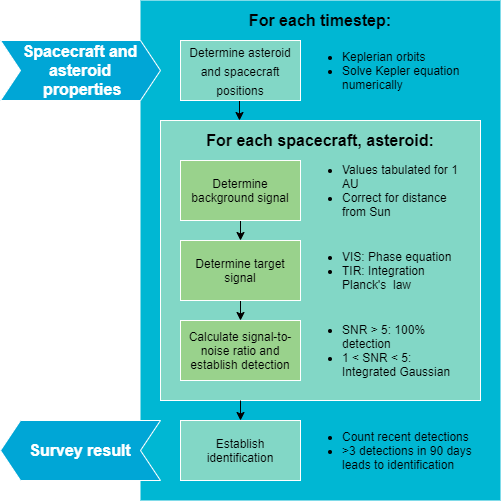
\includegraphics[width=0.7\textwidth]{img/simulation_overview.png}
 \caption{Overview of the simulation architecture and main loops.}
 \label{fig:simulation_overview}
\end{figure}

The architecture of the simulation is shown in \autoref{fig:simulation_overview}. On the top left, the main input parameters to the model are displayed. These are primarily the spacecraft and asteroid properties. Both of these consist of a full set of Keplerian orbital elements per spacecraft or asteroid. The asteroid properties furthermore include the albedo, size, and absolute magnitude of each asteroid; the spacecraft properties include which type of payload the spacecraft is carrying. \\

The simulation consists of a nested loop. Firstly, at the start of each timestep (the time between the timesteps is determined by the survey cadence), the positions of all asteroids and spacecraft are determined by propagation of their orbital elements. Then, in the inside loop, each spacecraft is checked against each asteroid to see if it can detect said asteroid. This is done through calculation of the signal-to-noise ratio (SNR). Lastly, as it is known which asteroids got succesfully detected by which spacecraft, it can be determined if asteroids have been identified. Then, at the end of the simulation, the result is a list of the asteroid population in addition to whether they have been detected, and if so, when. Of course, this data can be further processed.

\section{Implementation}

\section{Optimization Methods}

\section{Experimental Process}
